\documentclass{uofa-eng-assignment}
\usepackage[utf8]{inputenc}
\usepackage{geometry}
\geometry{
 a4paper,
 left=25.4mm,
 top=25.4mm,
 }
 \usepackage[spanish]{babel}
 \usepackage{graphicx} 
 \usepackage{float} 
 \usepackage{natbib}
 \usepackage{subcaption}
\usepackage{caption}
\usepackage{wrapfig}
 \usepackage{hyperref}
 \hypersetup{
    colorlinks=true,
    linkcolor=blue,
    filecolor=magenta,      
    urlcolor=cyan,
    pdftitle={Overleaf Example},
    pdfpagemode=FullScreen,
    }

\newcommand*{\name}{Natalia Opazo}

\newcommand*{\course}{1er Control MGR 622. “Evaluación de recursos acuáticos”  \\
Diplomado en Evaluación de Recursos Pesqueros}
%\newcommand*{\assignment}{Assignment 1}

\begin{document}

\maketitle

Considerando el archivo de datos asignado en:\\

\url{https://docs.google.com/spreadsheets/d/1aBkFS65_B4dH50NYrVMyAwPoXqbZFr7F/edit?usp=sharing&ouid=111551428972597948077&rtpof=true&sd=true}, ajuste el modelo de biomasa dinámica de Pella y Tomlinson considerando valores de p=1e-3, 1.0 y 3.0. Complete la tabla

\begin{table}[H]
\centering
\begin{tabular}{||l|c|c|c||}
\hline \hline
\textbf{p }                & \textbf{1e-3} & \textbf{1} &\textbf{3 }\\
\hline
\hline
\textbf{K }                &  2732.97    & 2594.131  & 2479.113  \\
\hline
\textbf{r }              &  0.3228347    &  0.5661019 & 1.081457  \\
\hline
\textbf{Sigma }            &  0.4520446    & 0.4568287  &  0.4992885 \\
\hline
\textbf{RMS }              &  324.4169    & 367.1356  & 422.2393  \\
\hline
\textbf{Brms }             & 1005.906     &  1297.065 & 1561.743  \\
\hline
\textbf{Frms }             & 0.3225122     & 0.283051  &  0.2703641 \\
\hline
\textbf{Log-verosimilitud }&  26.35727    &  26.62028 & 27.96508 \\
\hline
\end{tabular}
\end{table}

Preguntas: \\

1. ¿Son los tres modelos igualmente probables? Justifique su elección del mejor modelo. \\

Considerando el mejor modelo:\\

2. Comente brevemente respecto del ajuste del modelo y de sus residuales. Considere las gráficas apropiadas.\\

\begin{figure}[H]
    \centering
    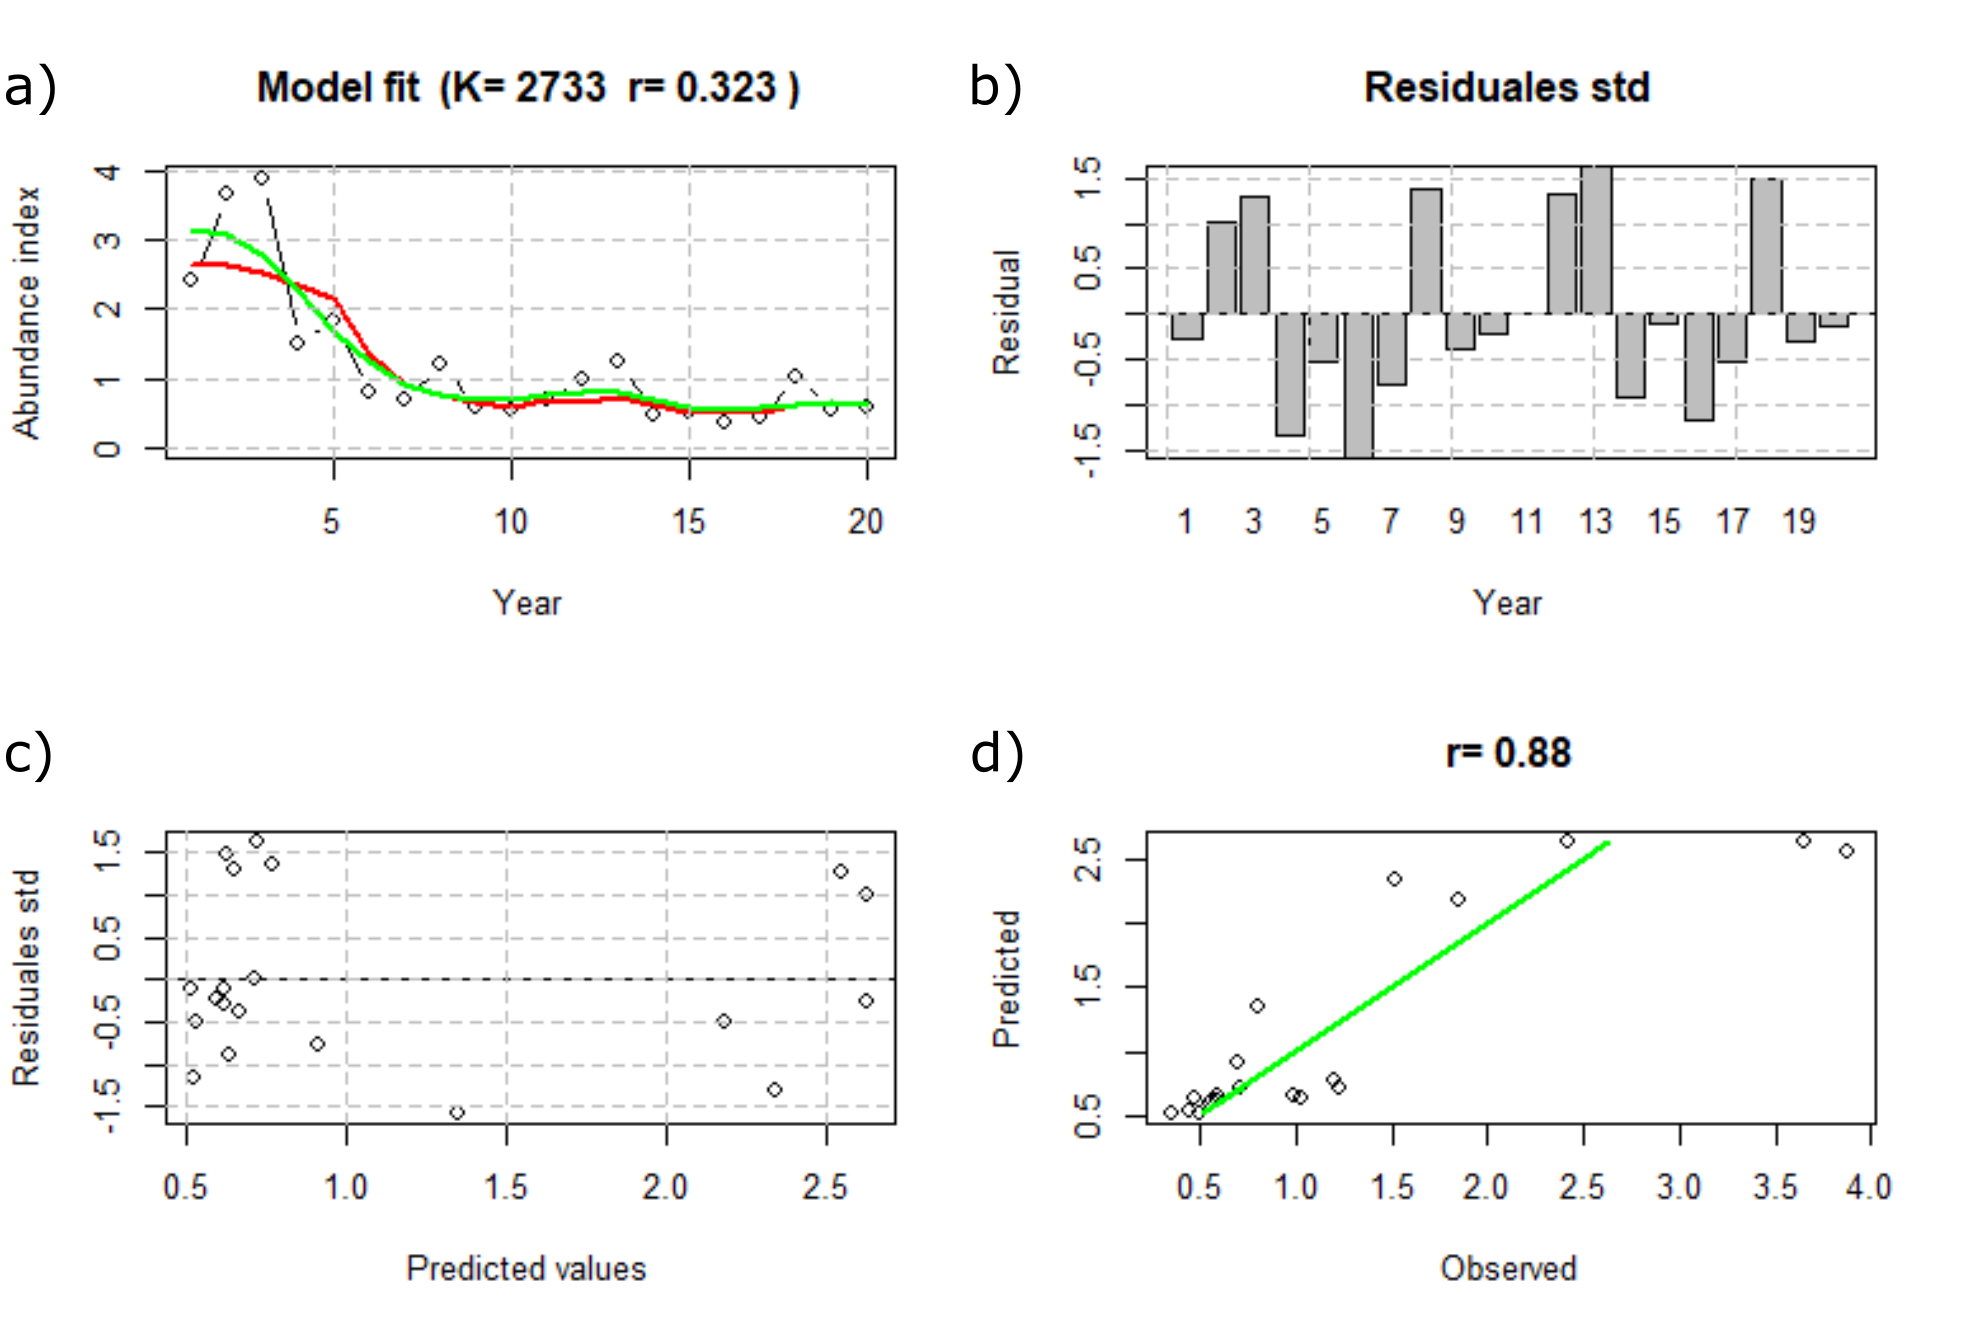
\includegraphics[scale=0.3]{1_1.png}
    \caption{Caption}
    \label{fig:1_1}
\end{figure}

\begin{figure}[H]
    \centering
    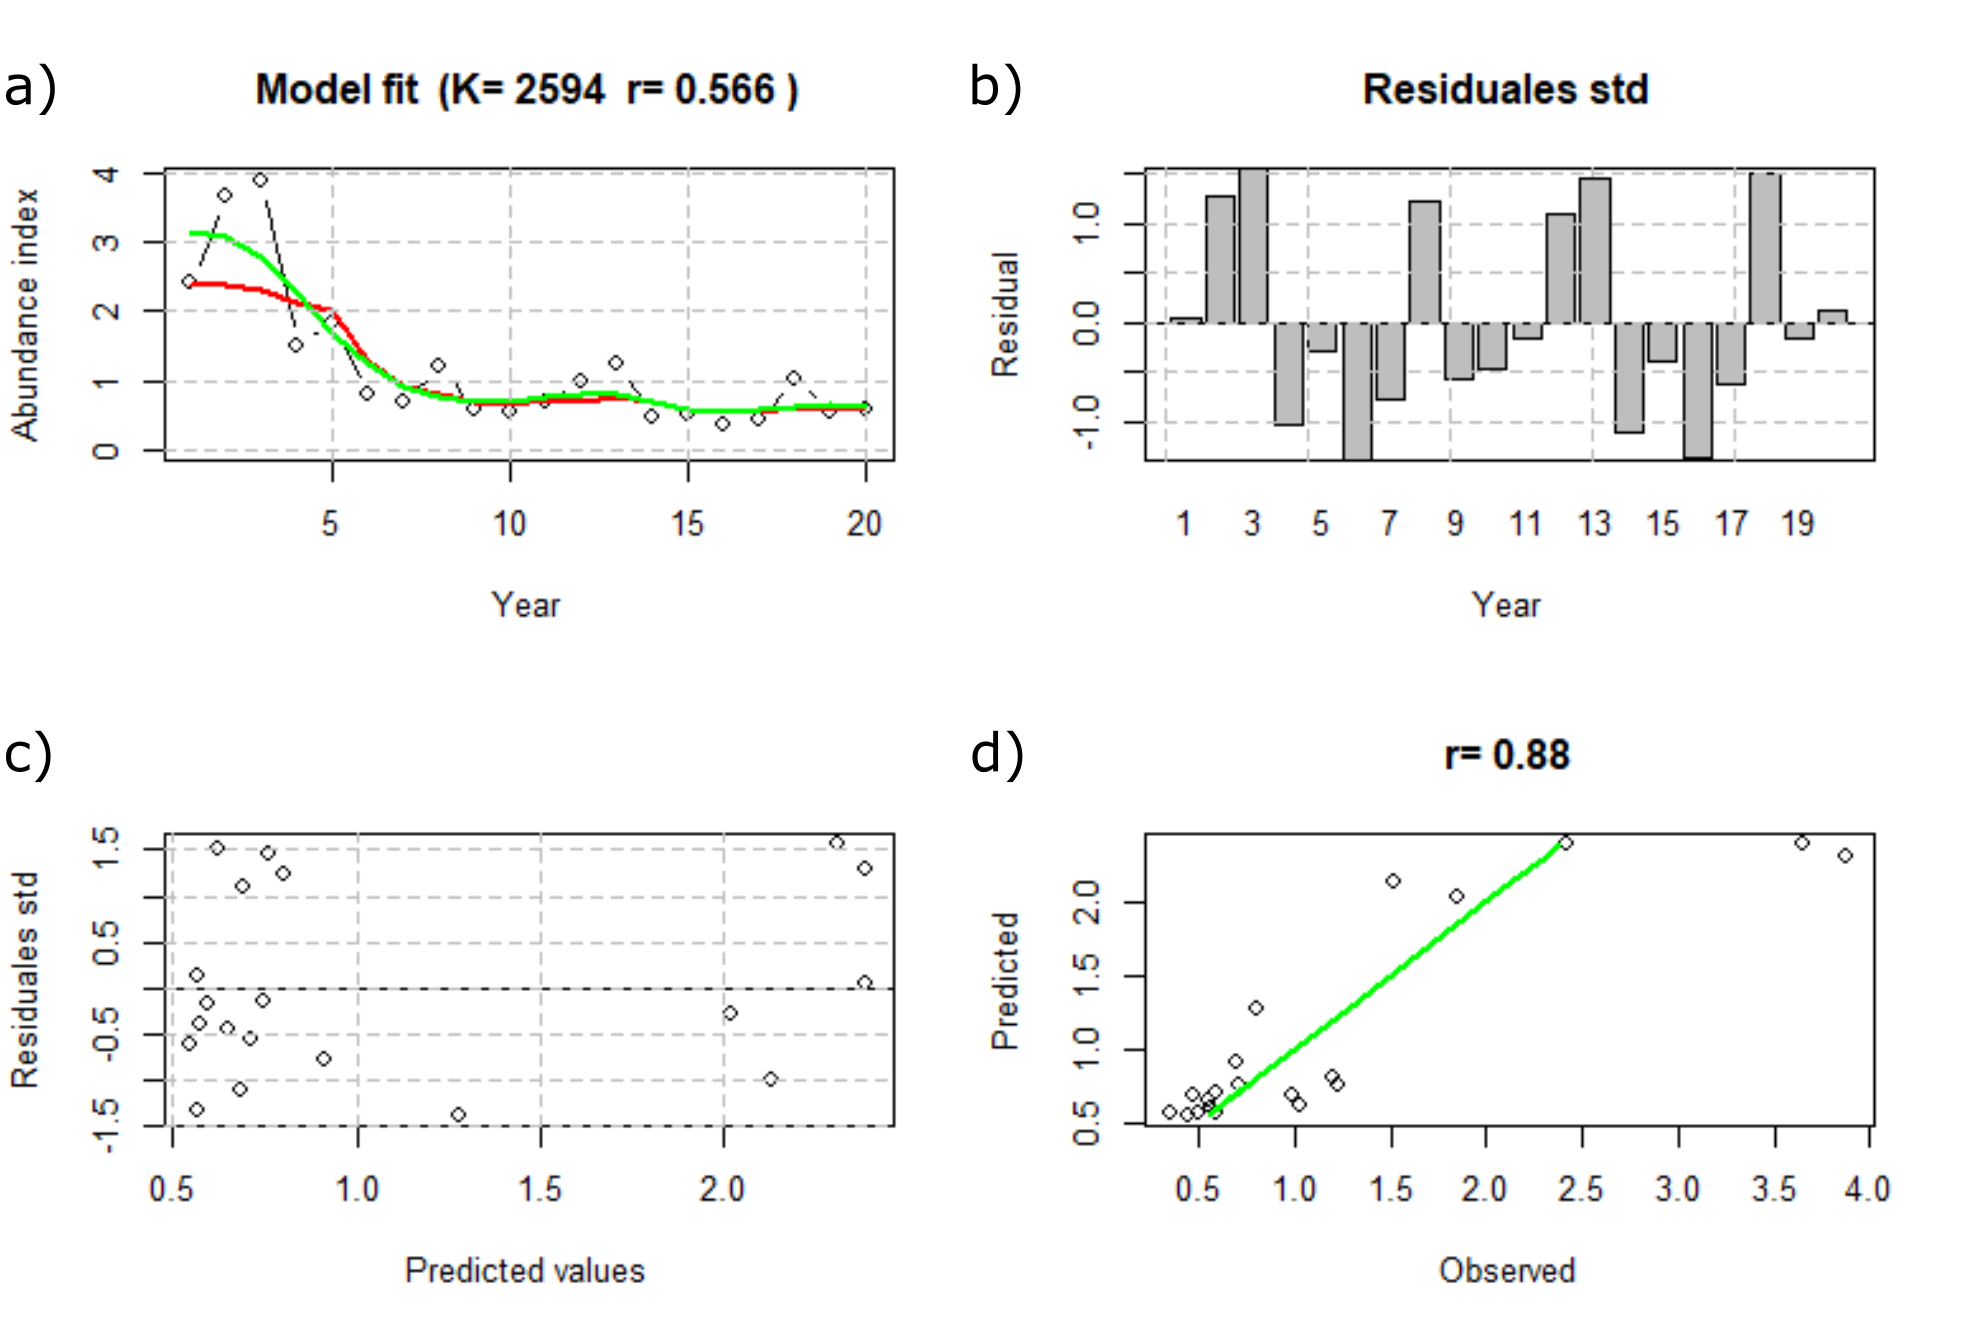
\includegraphics[scale=0.3]{2_1.png}
    \caption{Caption}
    \label{fig:2_1}
\end{figure}

\begin{figure}[H]
    \centering
    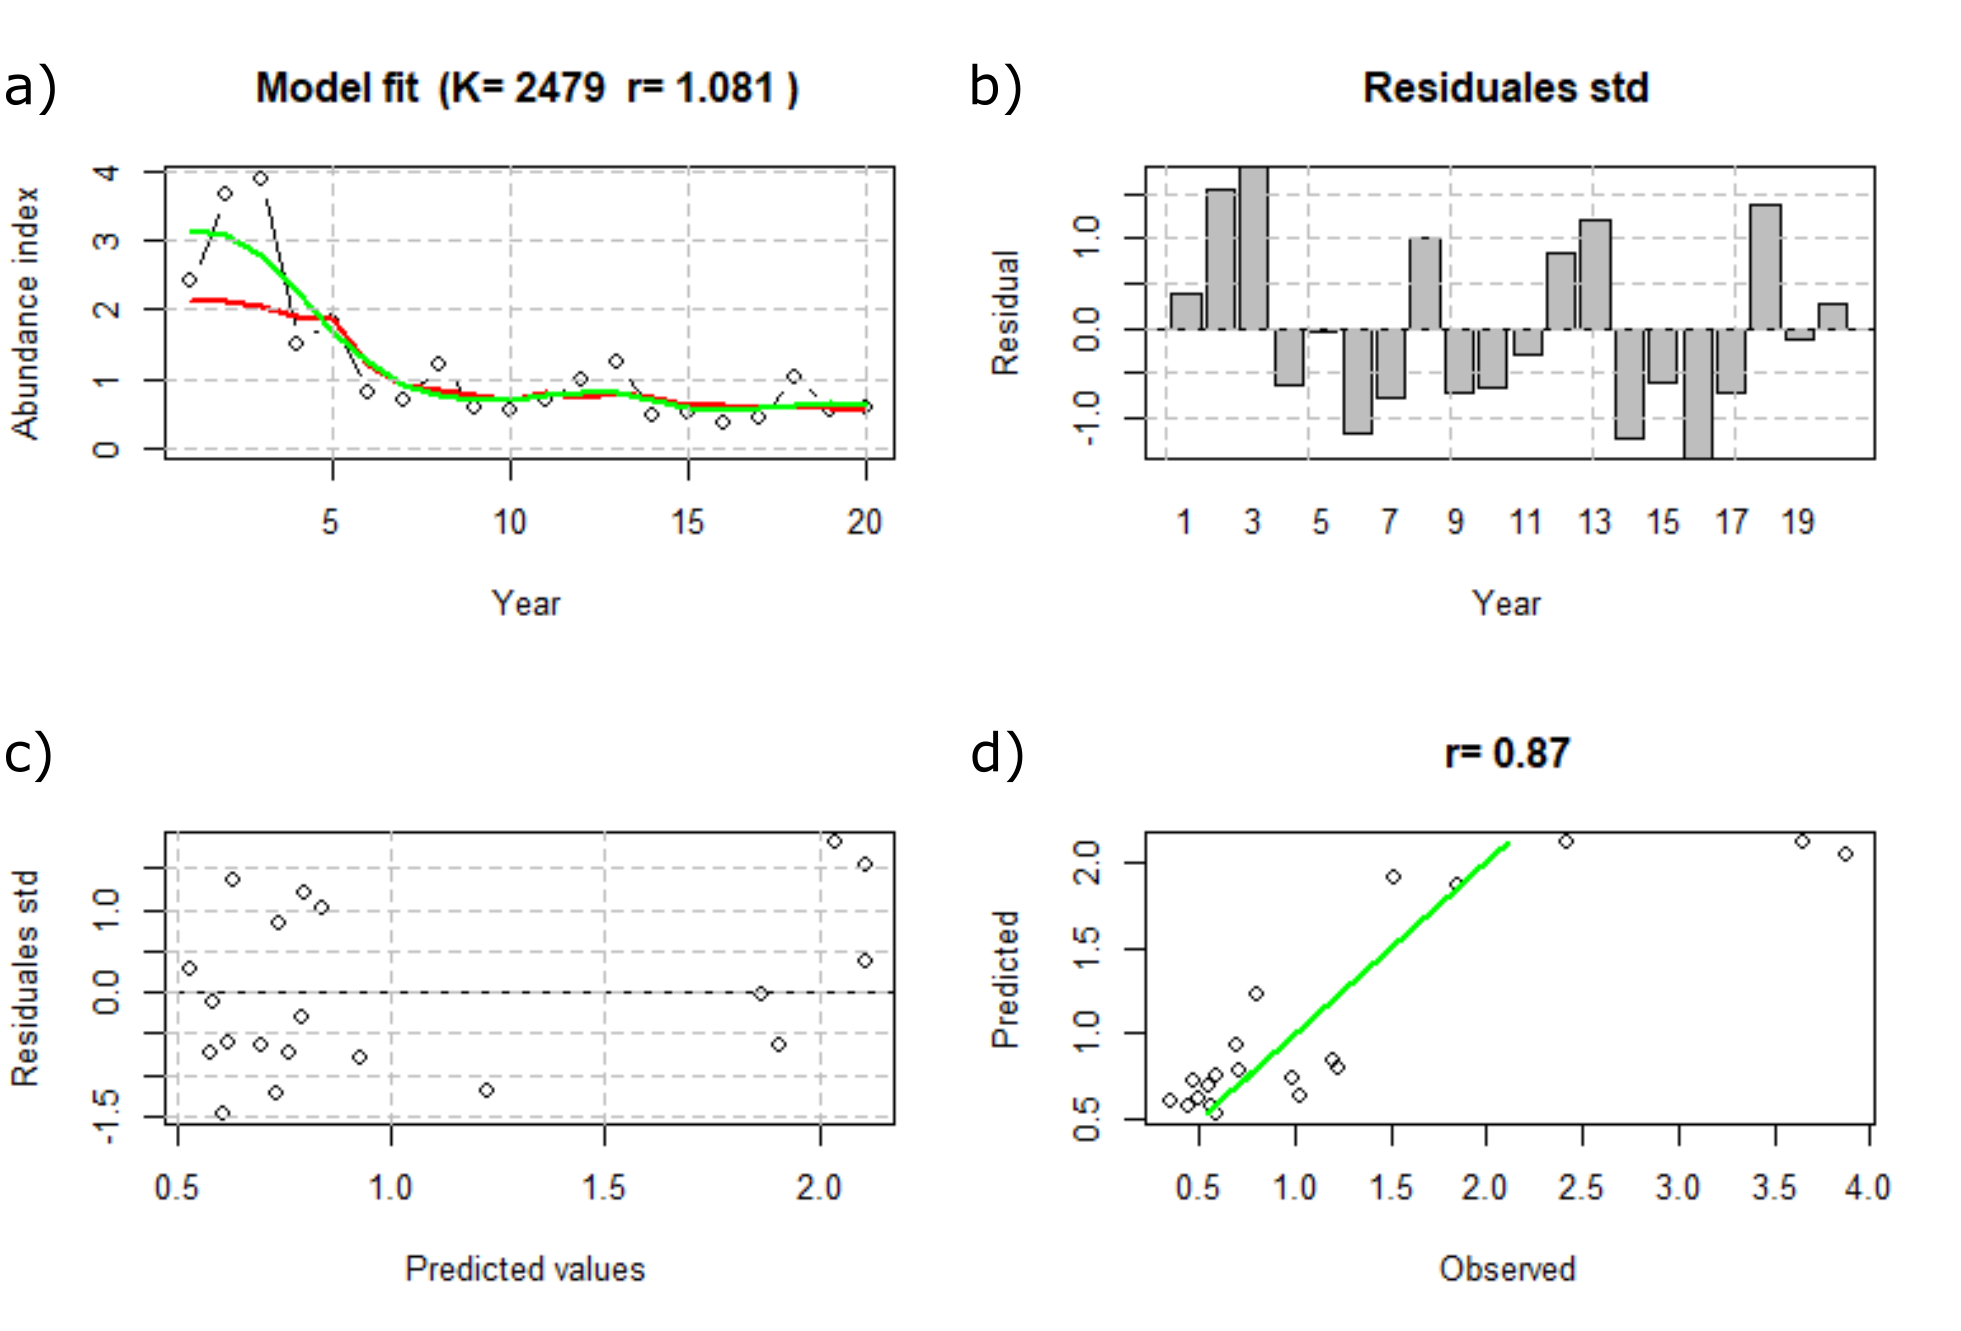
\includegraphics[scale=0.3]{3_1.png}
    \caption{Caption}
    \label{fig:3_1}
\end{figure}

3. Explique las causas de los cambios registrados en la población y establezca su diagnóstico. Considere solo las figuras necesarias.\\

\begin{figure}[H]
    \centering
    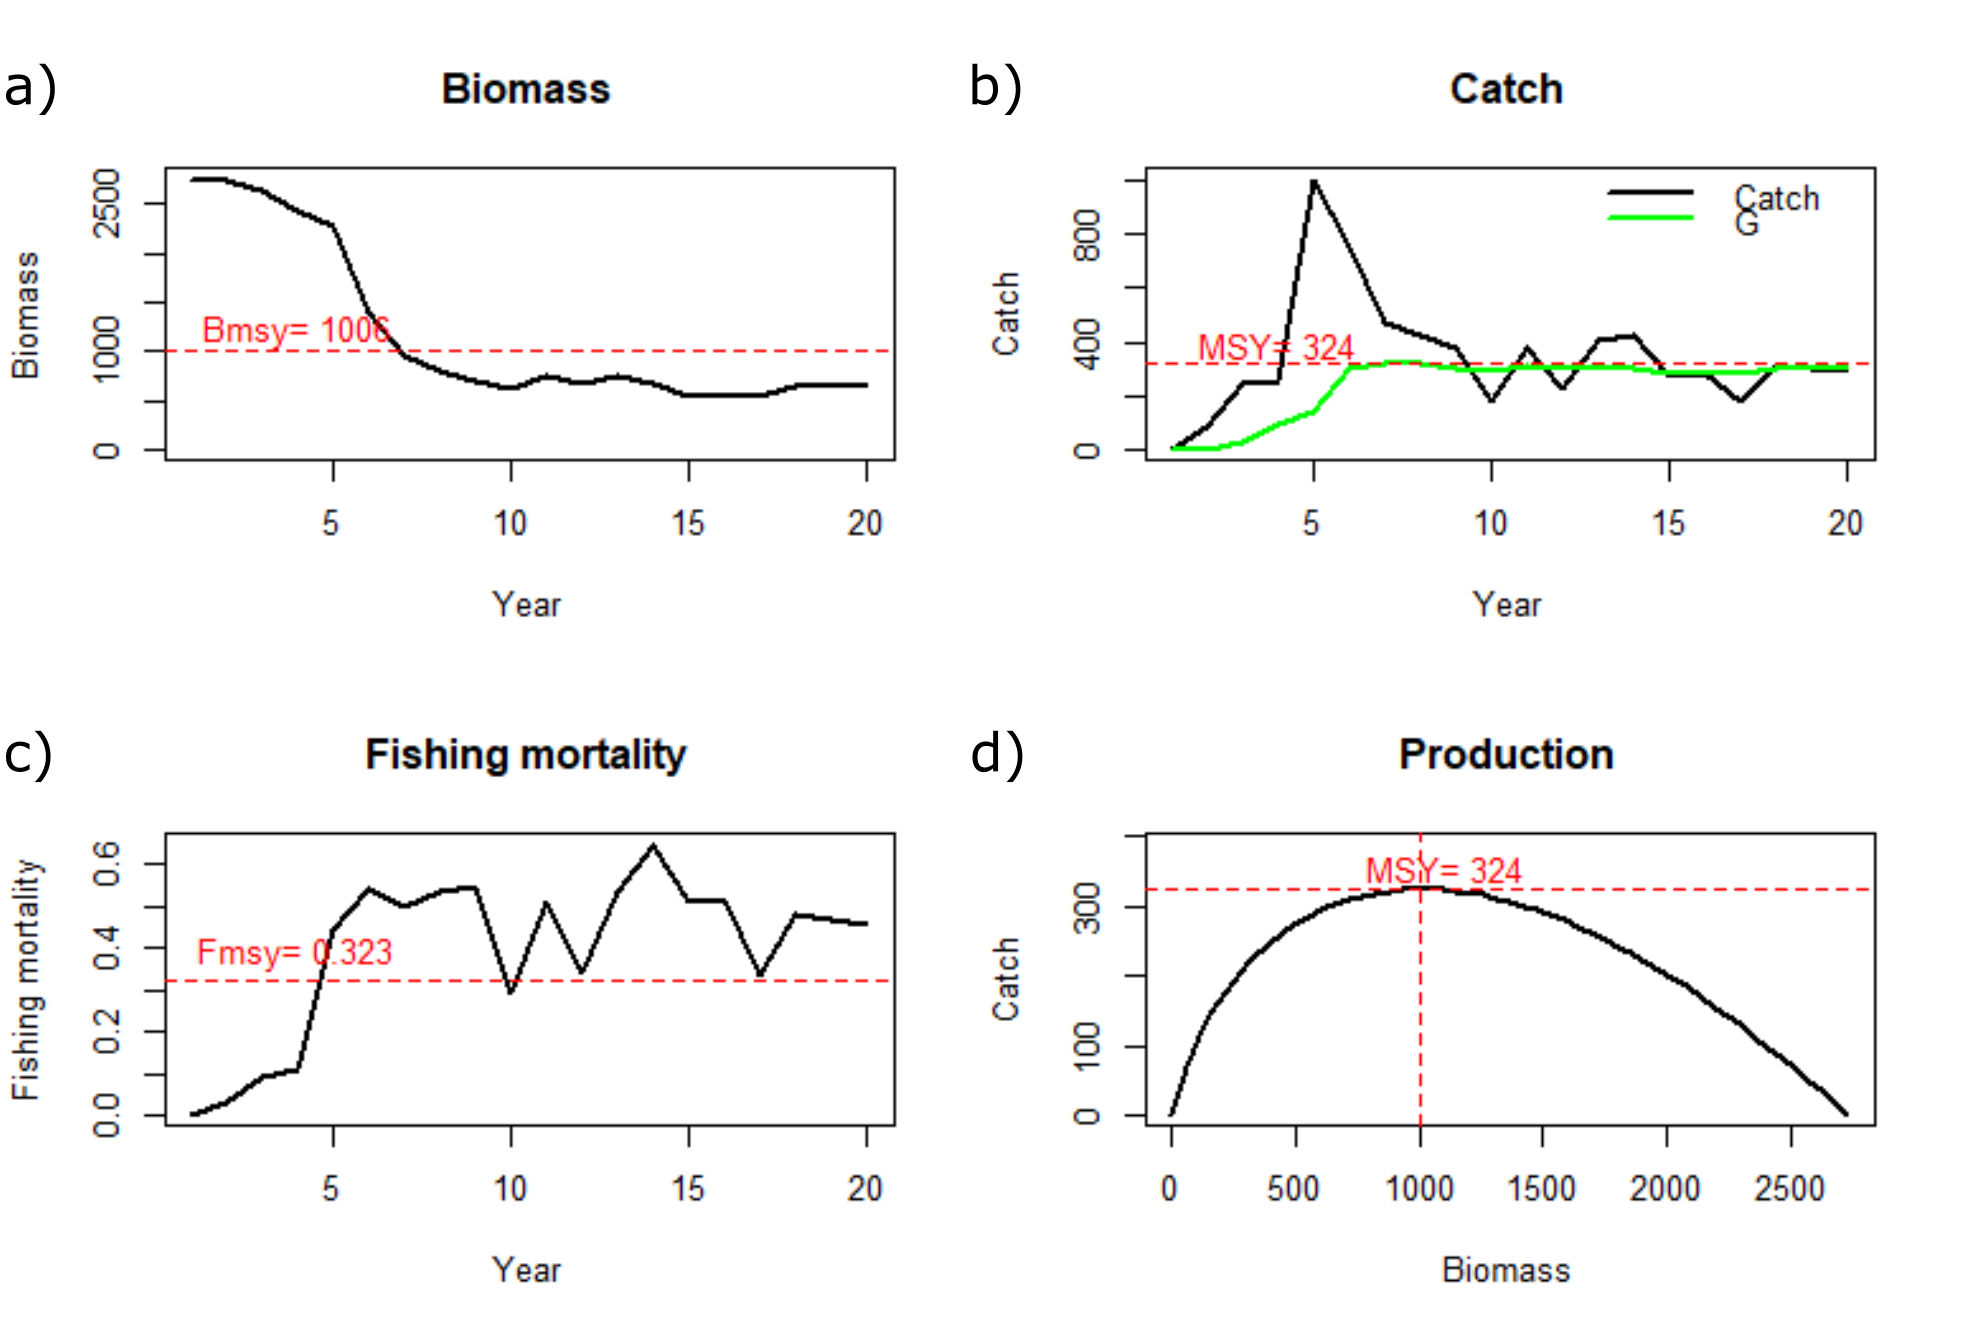
\includegraphics[scale=0.3]{1_2.png}
    \caption{Caption}
    \label{fig:1_2}
\end{figure}

\begin{figure}[H]
    \centering
    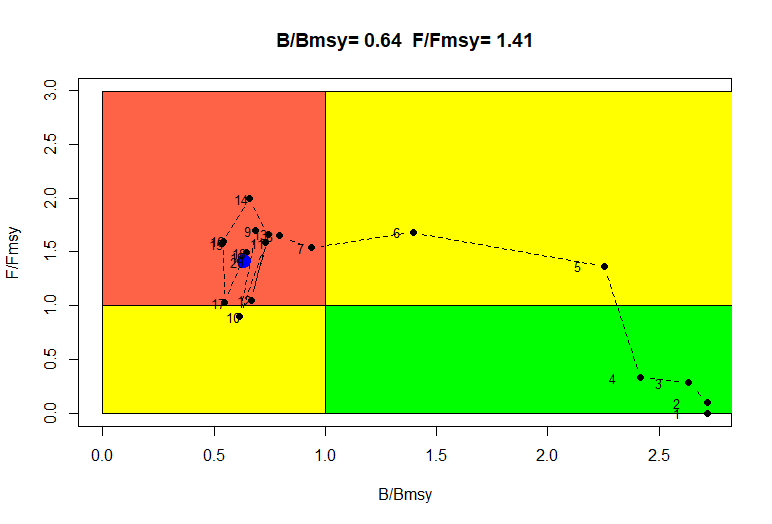
\includegraphics[scale=0.75]{1_3.png}
    \caption{Caption}
    \label{fig:1_3}
\end{figure}

\begin{figure}[H]
    \centering
    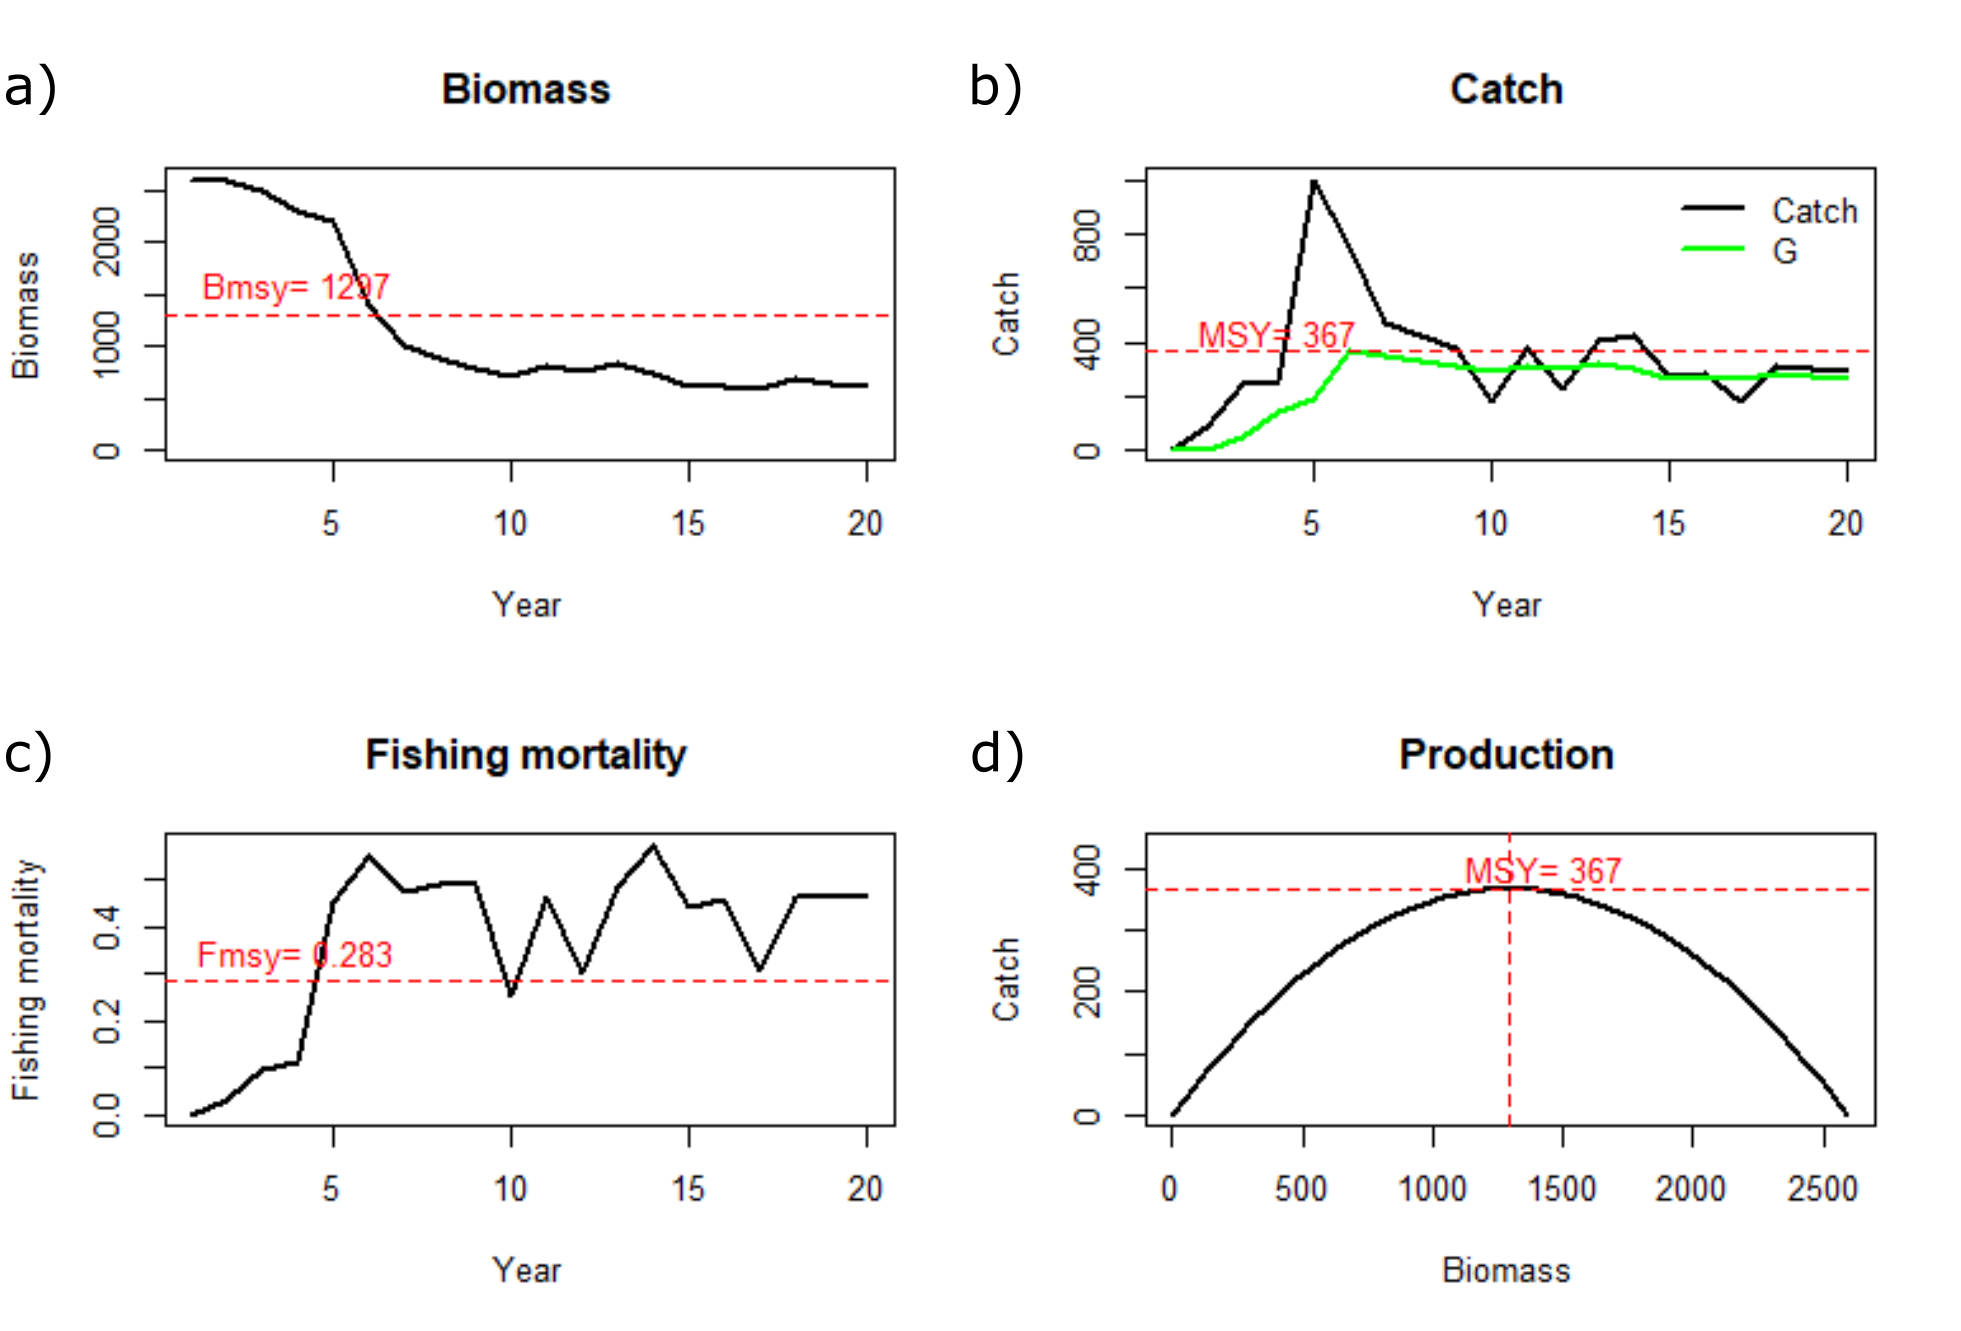
\includegraphics[scale=0.3]{2_2.png}
    \caption{Caption}
    \label{fig:2_2}
\end{figure}

\begin{figure}[H]
    \centering
    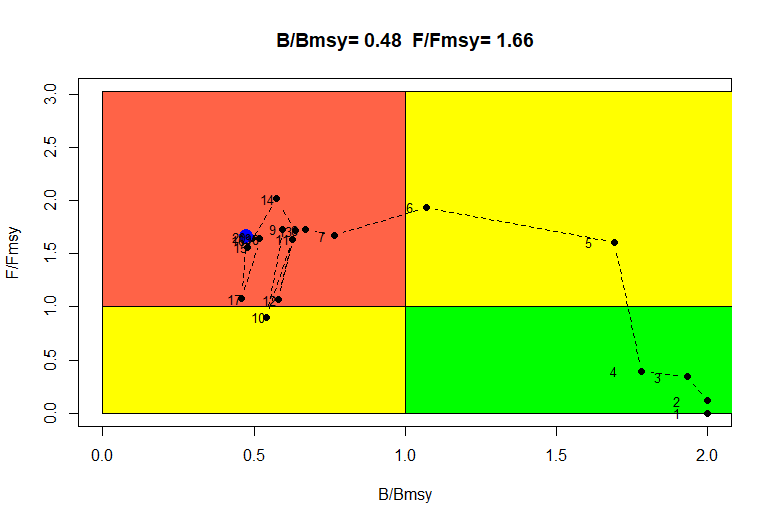
\includegraphics[scale=0.75]{2_3.png}
    \caption{Caption}
    \label{fig:2_3}
\end{figure}

\begin{figure}[H]
    \centering
    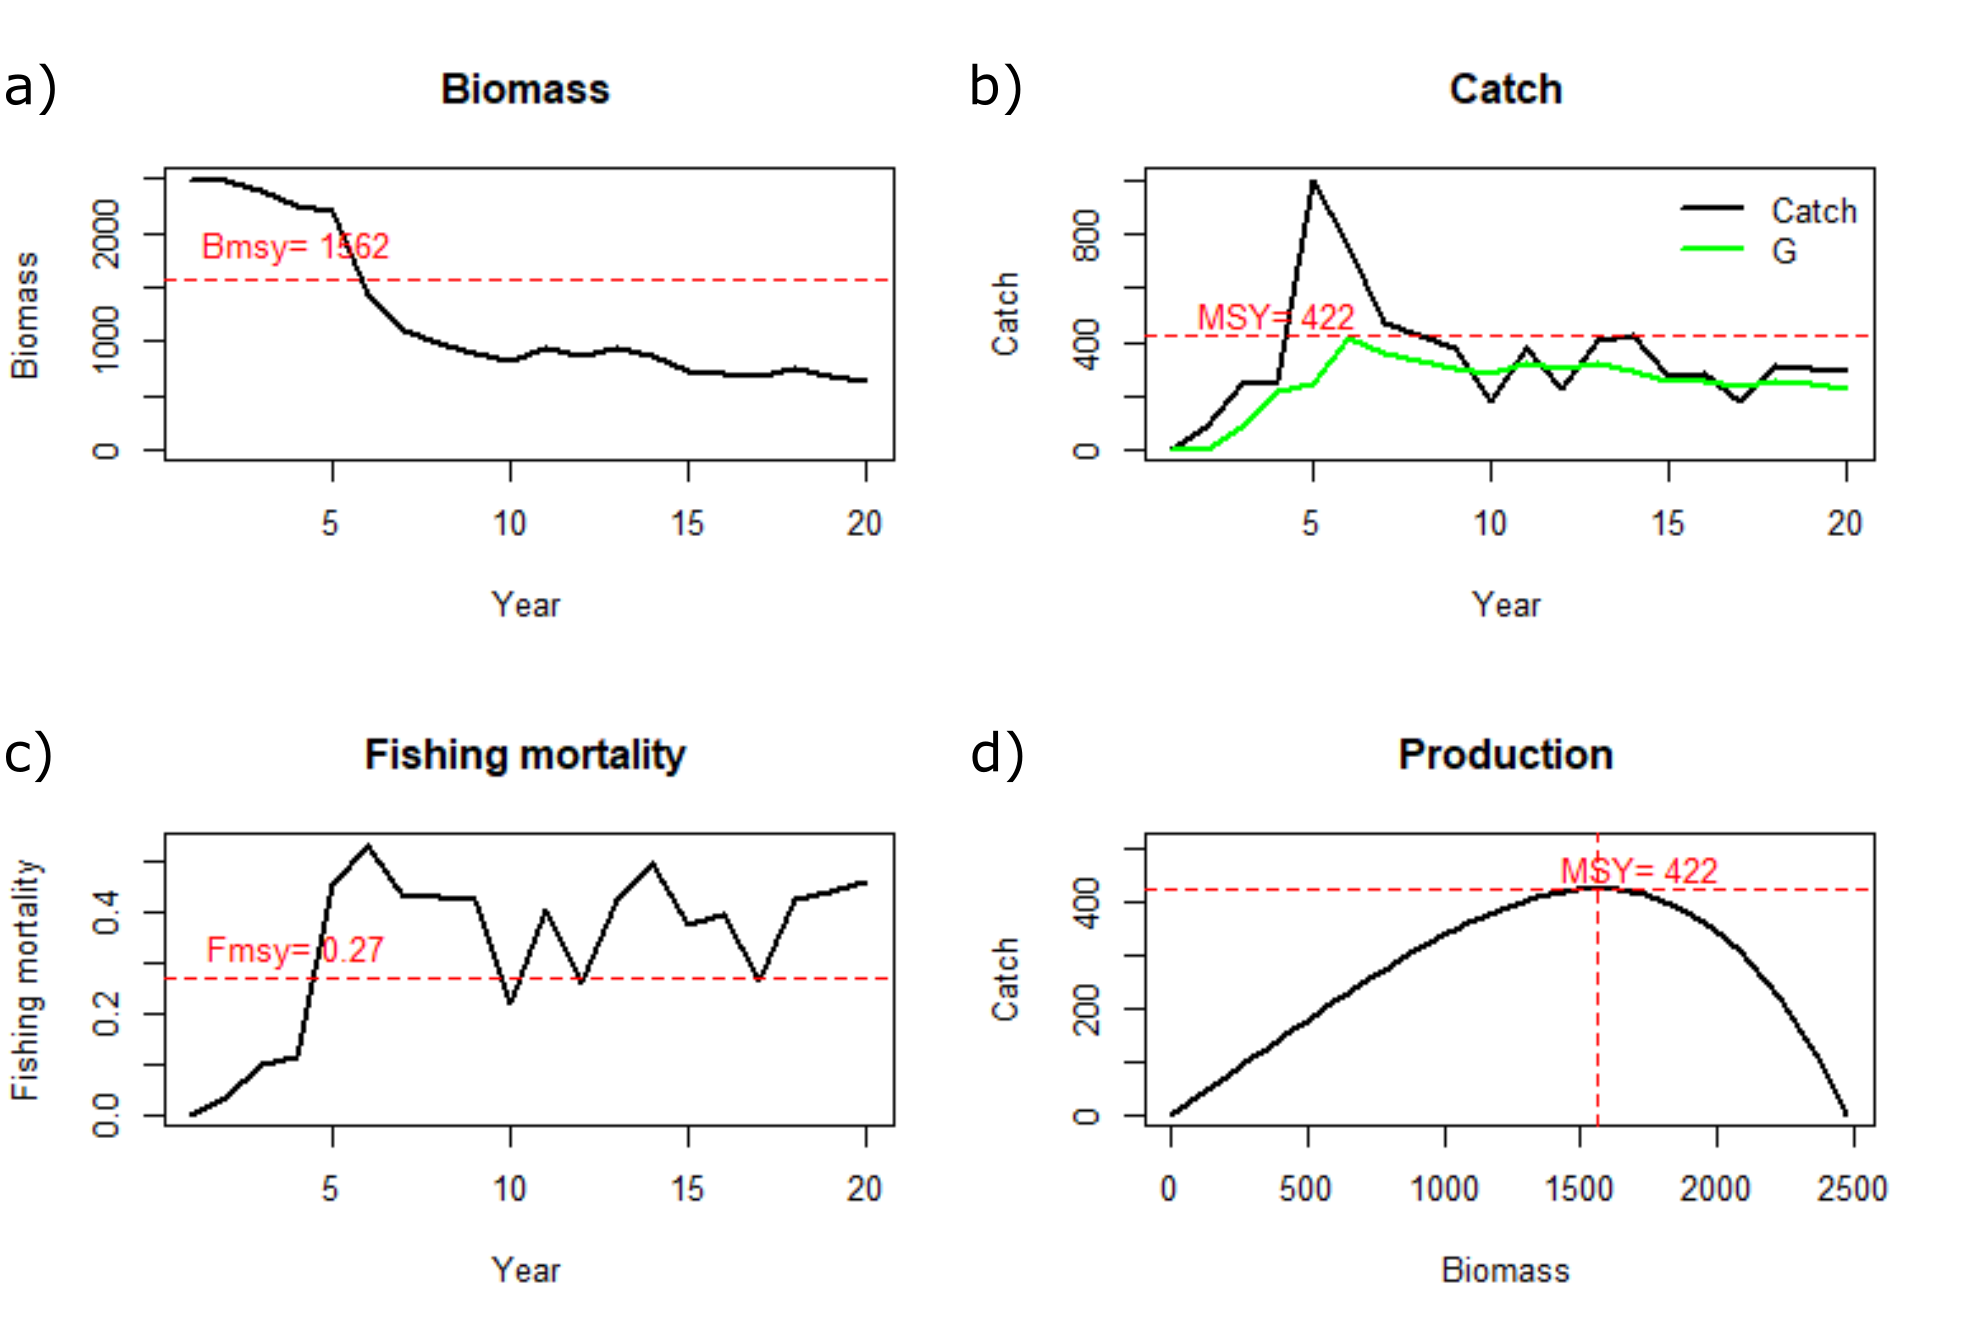
\includegraphics[scale=0.3]{3_2.png}
    \caption{Caption}
    \label{fig:3_2}
\end{figure}

\begin{figure}[H]
    \centering
    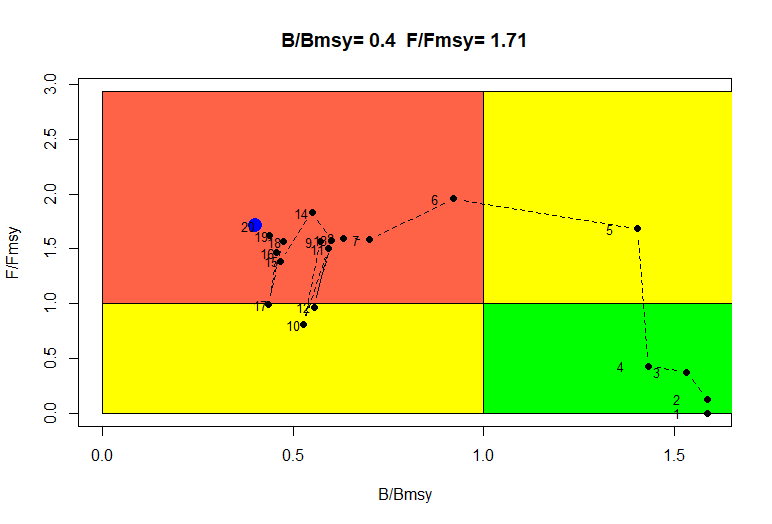
\includegraphics[scale=0.75]{3_3.png}
    \caption{Caption}
    \label{fig:3_3}
\end{figure}

4. Calcule el nivel de captura que permitiría mantener una biomasa del 40\% de la biomasa virginal en el largo plazo. Explique el procedimiento de cálculo y señale dicho valor en la gráfica respectiva.\\

\begin{figure}[H]
    \centering
    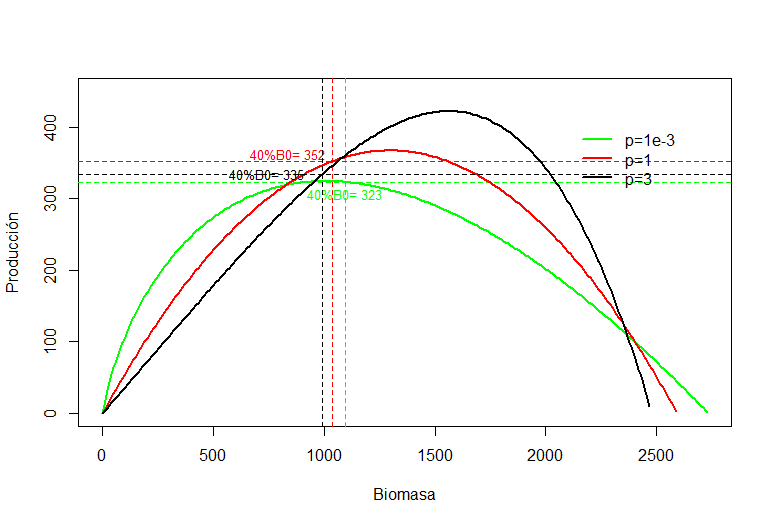
\includegraphics[scale=0.75]{ejer4.png}
    \caption{Caption}
    \label{fig:ejer4}
\end{figure}

\begin{equation}
    G1=r/p*B1*(1-(B1/K1)^p) 
\end{equation}

\begin{equation}
        40\%B0=0.4*K1
\end{equation}

\begin{equation}
     RMS40\%B0=r/p*Brms1_1*(1-(Brms1_1/K1)^p)
\end{equation}

\begin{itemize}
    \item p=1e-3\\
    RMS40\%B0=323.2283
    \item p=1 \\
    RMS40\%B0=352.4502
    \item p=3 \\
    RMS40\%B0=334.5956
   
\end{itemize}

5. Proyecte la biomasa al año 21 y calcule la captura que permitiría mantener a la población estable en este valor de biomasa. Compare con la Captura Biológicamente Aceptable que permitiría llevar a la biomasa al Brms (CBA = Frms*B). Comente sobre las implicancias para la pesquería establecer dicha CBA.\\

\begin{equation}
    Biom[21]=max(c(Biom[20] + r/rho*Biom[20]*(1-(Biom[20]/K)^rho) - Y[20],0.1))
\end{equation}

\begin{figure}[H]
    \centering
    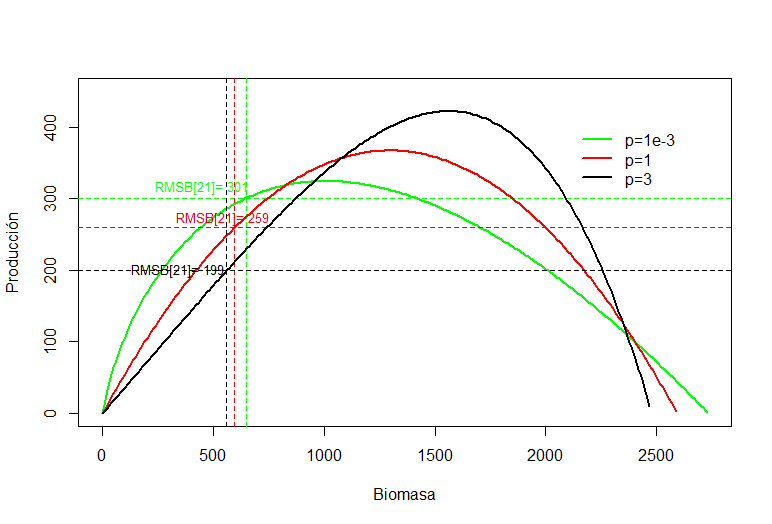
\includegraphics[scale=0.75]{ejer5.png}
    \caption{Caption}
    \label{fig:ejer5}
\end{figure}

\begin{itemize}
    \item p=1e-3\\
    Biom[21]=648.6148\\
    RMSB[21]=300.958
    \item p=1 \\
    Biom[21]=593.8721\\
    RMSB[21]=259.228
    \item p=3 \\
    Biom[21]=559.1106\\
    RMSB[21]=199.2393
  
\end{itemize}



6. Calcule el nivel de reducción del esfuerzo de pesca que permita recuperar a la población al valor Brms. Explique su procedimiento y comente respecto de lo obtenido en 5.

\section*{Anexos}

\begin{table}[H]
 \caption{Caption}
\begin{tabular}{llllllllll}
   & Año & CPUEobs & CPUEpred & Capturas  & Biomasa & F    & Produccion & B\_Bmsy & F\_Fmsy \\
1  & 1   & 2.42    & 2.63     & 0         & 2733    & 0    & 0          & 2.72    & 0       \\
2  & 2   & 3.66    & 2.63     & 86.14021  & 2733    & 0.03 & 0          & 2.72    & 0.1     \\
3  & 3   & 3.88    & 2.55     & 242.64    & 2647    & 0.09 & 27         & 2.63    & 0.28    \\
4  & 4   & 1.52    & 2.34     & 258.11201 & 2432    & 0.11 & 92         & 2.42    & 0.33    \\
5  & 5   & 1.84    & 2.18     & 999.86165 & 2265    & 0.44 & 137        & 2.25    & 1.37    \\
6  & 6   & 0.8     & 1.35     & 760.42097 & 1403    & 0.54 & 302        & 1.39    & 1.68    \\
7  & 7   & 0.7     & 0.91     & 468.50413 & 944     & 0.5  & 324        & 0.94    & 1.54    \\
8  & 8   & 1.2     & 0.77     & 425.35434 & 799     & 0.53 & 317        & 0.79    & 1.65    \\
9  & 9   & 0.59    & 0.66     & 378.27127 & 691     & 0.55 & 307        & 0.69    & 1.7     \\
10 & 10  & 0.55    & 0.6      & 178.79097 & 619     & 0.29 & 297        & 0.62    & 0.9     \\
11 & 11  & 0.71    & 0.71     & 376.66054 & 737     & 0.51 & 312        & 0.73    & 1.58    \\
12 & 12  & 0.99    & 0.65     & 227.23875 & 672     & 0.34 & 304        & 0.67    & 1.05    \\
13 & 13  & 1.23    & 0.72     & 401.44091 & 749     & 0.54 & 313        & 0.74    & 1.66    \\
14 & 14  & 0.47    & 0.64     & 424.64304 & 660     & 0.64 & 303        & 0.66    & 1.99    \\
15 & 15  & 0.5     & 0.52     & 273.72956 & 538     & 0.51 & 282        & 0.54    & 1.58    \\
16 & 16  & 0.36    & 0.53     & 281.94292 & 547     & 0.52 & 284        & 0.54    & 1.6     \\
17 & 17  & 0.45    & 0.53     & 181.80895 & 549     & 0.33 & 284        & 0.55    & 1.03    \\
18 & 18  & 1.02    & 0.63     & 312.78066 & 651     & 0.48 & 301        & 0.65    & 1.49    \\
19 & 19  & 0.56    & 0.62     & 300.11431 & 640     & 0.47 & 300        & 0.64    & 1.46    \\
20 & 20  & 0.59    & 0.61     & 290       & 639     & 0.45 & 300        & 0.64    & 1.41   
\end{tabular}
\end{table}

\begin{table}[H]
\caption{Caption}
\begin{tabular}{lllllllll}
Año & CPUEobs & CPUEpred & Capturas  & Biomasa & F    & Produccion & B\_Bmsy & F\_Fmsy \\
1   & 2.42    & 2.39     & 0         & 2594    & 0    & 0          & 2       & 0       \\
2   & 3.66    & 2.39     & 86.14021  & 2594    & 0.03 & 0          & 2       & 0.12    \\
3   & 3.88    & 2.31     & 242.64    & 2508    & 0.1  & 47         & 1.93    & 0.34    \\
4   & 1.52    & 2.13     & 258.11201 & 2312    & 0.11 & 142        & 1.78    & 0.39    \\
5   & 1.84    & 2.02     & 999.86165 & 2197    & 0.46 & 191        & 1.69    & 1.61    \\
6   & 0.8     & 1.28     & 760.42097 & 1387    & 0.55 & 365        & 1.07    & 1.94    \\
7   & 0.7     & 0.91     & 468.50413 & 992     & 0.47 & 347        & 0.76    & 1.67    \\
8   & 1.2     & 0.8      & 425.35434 & 871     & 0.49 & 327        & 0.67    & 1.73    \\
9   & 0.59    & 0.71     & 378.27127 & 773     & 0.49 & 307        & 0.6     & 1.73    \\
10  & 0.55    & 0.65     & 178.79097 & 701     & 0.25 & 290        & 0.54    & 0.9     \\
11  & 0.71    & 0.75     & 376.66054 & 812     & 0.46 & 316        & 0.63    & 1.64    \\
12  & 0.99    & 0.69     & 227.23875 & 752     & 0.3  & 302        & 0.58    & 1.07    \\
13  & 1.23    & 0.76     & 401.44091 & 827     & 0.49 & 319        & 0.64    & 1.72    \\
14  & 0.47    & 0.68     & 424.64304 & 744     & 0.57 & 300        & 0.57    & 2.02    \\
15  & 0.5     & 0.57     & 273.72956 & 620     & 0.44 & 267        & 0.48    & 1.56    \\
16  & 0.36    & 0.56     & 281.94292 & 613     & 0.46 & 265        & 0.47    & 1.63    \\
17  & 0.45    & 0.55     & 181.80895 & 596     & 0.31 & 260        & 0.46    & 1.08    \\
18  & 1.02    & 0.62     & 312.78066 & 674     & 0.46 & 282        & 0.52    & 1.64    \\
19  & 0.56    & 0.59     & 300.11431 & 644     & 0.47 & 274        & 0.5     & 1.65    \\
20  & 0.59    & 0.57     & 290       & 618     & 0.47 & 266        & 0.48    & 1.66   
\end{tabular}
\end{table}

\begin{table}[H]
 \caption{Caption}
\begin{tabular}{llllllllll}
   & Año & CPUEobs & CPUEpred & Capturas  & Biomasa & F    & Produccion & B\_Bmsy & F\_Fmsy \\
1  & 1   & 2.42    & 2.11     & 0         & 2479    & 0    & 0          & 1.59    & 0       \\
2  & 2   & 3.66    & 2.11     & 86.14021  & 2479    & 0.03 & 0          & 1.59    & 0.13    \\
3  & 3   & 3.88    & 2.04     & 242.64    & 2393    & 0.1  & 87         & 1.53    & 0.38    \\
4  & 4   & 1.52    & 1.91     & 258.11201 & 2237    & 0.12 & 214        & 1.43    & 0.43    \\
5  & 5   & 1.84    & 1.87     & 999.86165 & 2193    & 0.46 & 243        & 1.4     & 1.69    \\
6  & 6   & 0.8     & 1.22     & 760.42097 & 1436    & 0.53 & 417        & 0.92    & 1.96    \\
7  & 7   & 0.7     & 0.93     & 468.50413 & 1093    & 0.43 & 360        & 0.7     & 1.59    \\
8  & 8   & 1.2     & 0.84     & 425.35434 & 985     & 0.43 & 333        & 0.63    & 1.6     \\
9  & 9   & 0.59    & 0.76     & 378.27127 & 892     & 0.42 & 307        & 0.57    & 1.57    \\
10 & 10  & 0.55    & 0.7      & 178.79097 & 821     & 0.22 & 285        & 0.53    & 0.81    \\
11 & 11  & 0.71    & 0.79     & 376.66054 & 927     & 0.41 & 317        & 0.59    & 1.5     \\
12 & 12  & 0.99    & 0.74     & 227.23875 & 867     & 0.26 & 299        & 0.56    & 0.97    \\
13 & 13  & 1.23    & 0.8      & 401.44091 & 939     & 0.43 & 320        & 0.6     & 1.58    \\
14 & 14  & 0.47    & 0.73     & 424.64304 & 858     & 0.5  & 296        & 0.55    & 1.83    \\
15 & 15  & 0.5     & 0.62     & 273.72956 & 729     & 0.38 & 256        & 0.47    & 1.39    \\
16 & 16  & 0.36    & 0.61     & 281.94292 & 712     & 0.4  & 251        & 0.46    & 1.47    \\
17 & 17  & 0.45    & 0.58     & 181.80895 & 680     & 0.27 & 240        & 0.44    & 0.99    \\
18 & 18  & 1.02    & 0.63     & 312.78066 & 739     & 0.42 & 259        & 0.47    & 1.57    \\
19 & 19  & 0.56    & 0.58     & 300.11431 & 685     & 0.44 & 242        & 0.44    & 1.62    \\
20 & 20  & 0.59    & 0.53     & 290       & 627     & 0.46 & 222        & 0.4     & 1.71   
\end{tabular}
\end{table}

\end{document}
